\section{Search}
Both of the search algorithms we implemented perform a completely new search for solutions every game frame and no information is kept between frames.

\subsection{UCT Search}
UCT, Upper Confidence bounds for Trees, is the most popular Monte-Carlo Tree Search algorithm for playing games that are otherwise hard for computers to handle. \cite{mcts}

UCT, or indeed any other search algorithm, would however not be able to handle the huge branching factor of RTS games if they were to consider all possible combinations of actions.
This algorithm has recently seen success in the game of Go, but more relevant to our topic, also been applied to games such as Arimaa, and even RTS games (in \cite{portfolio} and \cite{wargusuct}).
Arimaa is interesting because it has an average branching factor of 17000, which is large when compared to chess, with 35, or Go, with 250.
To manage the branching factor in Arimaa in \cite{arimaa}, the author tried something like the UnitAction presented here in \ref{actiongeneration}, basically deciding the order for each unit in turn, one unit per node in the game tree.

In our implementation of UCT we use the UnitAction branching method, LTD2 state evaluation and for move orderings we simply consider attacking units in range before moving.
For a complete review of how UCT works we refer to \cite{mcts}.

\subsection{ABCD Search}
%move to related work?
In \cite{abcd}, an extended version of alpha-beta pruning, which is a well-known searching algorithm, was used for micromanagement. 
They were able to find good solutions for 8 v.s. 8 unit scenarios in 5 ms, achieving around a 80\% win rate against their best script.

In order to use alpha-beta algorithm it is necessary to separates the player's actions and its opponents action. We used the method \texttt{PlayerActionSubset} to do so. 

The children of a node are the restriction of its children to only one player set of actions:
$$
S_{A|p} = \{A \in S_A | \forall a \in A, a \text{ is an action performed by $p$}\}
$$
Algorithm \ref{algABCD} presents the ABCD algorithm.
The main distinction with the ``classic'' alpha-beta algorithm is that there is not a perfect alternation between $MAX$ and $MIN$. Once a state has no possible actions, we move in time until one of the players can perform an action. 
Figure \ref{figABCD} shows an example of such a tree: once we've reached a state where no action can be made for both player, we advance in time. In this new frame, there is an action for $MAX$. Therefore it is still he who is considered as the current player.

\begin{figure}[h!t]
    \begin{algorithm}[ABCD (Alpha-Beta Considering Durations)]
Let $s_0$ be the root node, $MAX$ be the player and $MIN$ the opponent. The algorithm return the best move compute by $ABCD(s_0,d_{max},-\infty,+\infty,MAX)$ where: \ \\

        \textbf{Function} $ABCD(s,d,\alpha,\beta,p)$:
        \begin{enum}
        \item \textbf{If} ($s$ is a terminal state) \textbf{Return} $LTD2(s)$
        \item \textbf{Else}
            \begin{enum}
            \item If $S_{A|p} \neq \emptyset$ 

            \begin{enum}
            \item \textbf{While} $S_{A|p} \neq \emptyset$
                \begin{enum}
                \item Pop $s_1$ from $S_{A|p}$ 
                \item Let $v = ABCD(s_1,d-1,\alpha,\beta,\bar{p})$
                \item \textbf{If} $p = MAX$ and $(v > \alpha)$ \textbf{then} $\alpha = v$
                \item \textbf{If} $p = MIN$ and $(v < \beta)$ \textbf{then} $\beta= v$
                \item \textbf{If} $\alpha \geq \beta$ \textbf{then break} 
                \end{enum}
            \item \textbf{Return} $(p = MAX) ? \alpha : \beta$ 
            \end{enum}
        \item \textbf{Else if} $S_{A|\bar{p}} \neq \emptyset$
            \begin{enum}
            \item \textbf{Return} $ABCD(s,d,\alpha,\beta,\bar{p})$
            \end{enum}
        \item \textbf{Else} 
            \begin{enum}
            \item Advance in time to state $s'$ for which $S'_A \neq \emptyset$
            \item \textbf{Return} $ABCD(s',d,\alpha,\beta,p)$
            \end{enum}
        \end{enum}
        \end{enum}
        \ \\
        And $s$ being considered as a \textbf{terminal state} if $d_{max}$ is reached, the time is elapsed or the state is a winning/loosing situation.
        \label{algABCD}
    \end{algorithm}
\end{figure}

\begin{figure}[h!t]
\centering
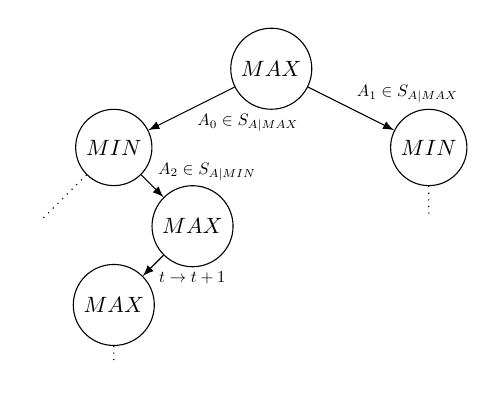
\begin{tikzpicture}[node distance = 1cm]
    \tikzstyle{node}=[circle,align=center,scale=0.8,draw]
    \tikzstyle{nodenotgen}=[circle,dotted,align=center,scale=0.8,draw]
    \tikzstyle{nodeterm}=[circle,fill=gray!30,align=center,scale=0.8,draw]
    \tikzstyle{link}=[->,thin,>=latex]
    
    \node[node] (s0) at (4,4) {$MAX$};

    \node[node] (s1) at (2,3) {$MIN$};
    \node[node] (s3) at (6,3) {$MIN$};

    \node[auto,scale=0.8] (s33) at (6,2) {};
    \draw[-,>=latex,dotted] (s3) to (s33);

    \node[auto,scale=0.8] (s4) at (1,2) {};
    \node[node] (s6) at (3,2) {$MAX$};

    \node[node] (s7) at (2,1) {$MAX$};

    \node[auto,scale=0.8] (s8) at (2,0.2) {};
    
    \draw[link] (s0) to node [auto,scale=0.6] {$A_0 \in S_{A|MAX}$} (s1); 
    \draw[link] (s0) to node [auto,scale=0.6] {$A_1 \in S_{A|MAX}$} (s3);
    \draw[-,>=latex,dotted] (s1) to (s4);
    \draw[link] (s1) to node [auto,scale=0.6] {$A_2 \in S_{A|MIN}$} (s6);
    \draw[link] (s6) to node [auto,scale=0.6] {$t \rightarrow t+1$} (s7);
    \draw[-,>=latex,dotted] (s7) to (s8);
    

\end{tikzpicture}
    \caption{Example of a graph constructed by the ABCD-algorithm}
    \label{figABCD}
\end{figure}

